\section{Architecture}
\label{s:arch}



\begin{figure}[h!]
\begin{center}
   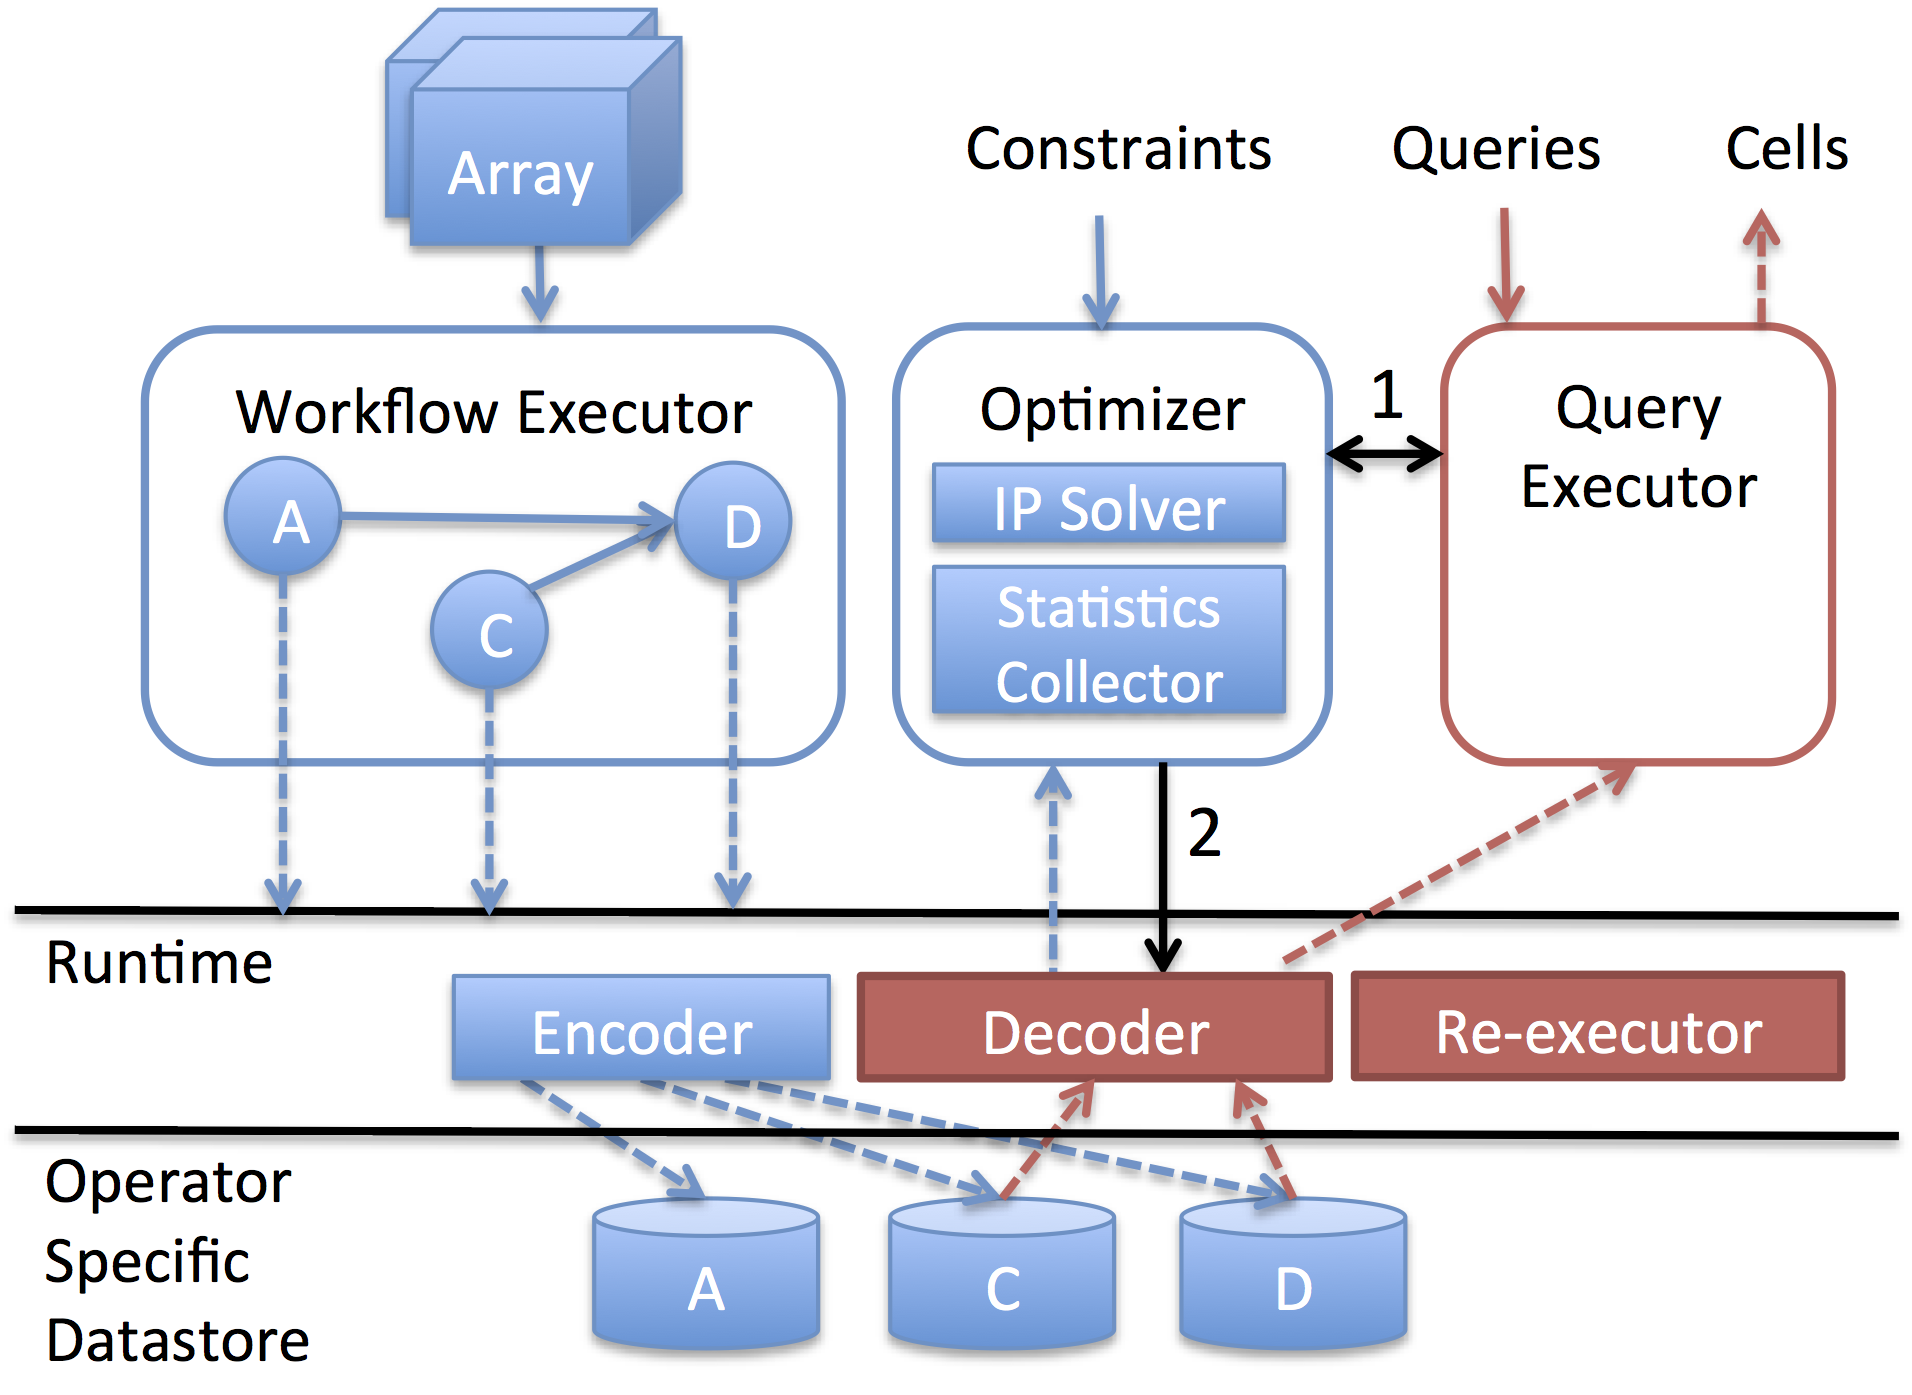
\includegraphics[width=2.9in,natwidth=6.38in,natheight=4.66in]{figures/arch.png}
\caption{The \sys{} architecture.  }
\vspace{-.1in} 
\label{f:arch}
\end{center}
\end{figure}

\sys{} records and stores lineage data at workflow runtime and uses it
to efficiently execute lineage queries.  The input to \sys{} is a
workflow specification (the graph in {\it Workflow Executor}),
constraints on the amount of storage that can be devoted to lineage
tracking, and a sample lineage query workload that the user expects to run.  \sys{} optimally decides
the type of lineage that each operator in the workflow will
generate ( the {\it lineage strategy}) in order to maximize the
performance of the query workload performance.


Figure \ref{f:arch} shows the system architecture.  The solid and
dashed arrows indicate the control and data flow, respectively.  Users
interact with \sys{} by defining and executing workflows ({\it
  Workflow Executor}), specifying constraints to the {\it Optimizer},
and running lineage queries ({\it Query Executor}).  The operators
in the workflow specify a list of the types of lineage
(described in Section~\ref{s:storagemodel}) that each operator can
generate, which defines the set of optimization possibilities.  

Each
operator initially generates black-box lineage (i.e., just records the names of the inputs it processes) but over time
changes its strategy through optimization.  As operators 
process data, they send lineage to the {\it
  Runtime}, which uses
the {\it Encoder} to serialize the lineage before writing it to
{\it Operator Specific Datastores}.  The {\it Runtime} may also send
lineage and other statistics to the {\it Optimizer}, which
calculates  statistics such as the amount of
lineage that each operator generates.  \sys{} periodically runs the
{\it Optimizer}, which uses an {\it Integer Programming Solver} to compute
the new lineage strategy.  On the right side, the {\it Query
  Executor} compiles lineage queries into query plans that join the
query with lineage data.  The {\it Executor} requests lineage
from the {\it Runtime}, which  reads and decodes  stored
lineage, uses the {\it Re-executor} to re-run the operators, and
 sends statistics (e.g., query fanout and
fanin) to the optimizer to refine future optimizations.

Given this  overview, we now describe the data model and structure of lineage
queries (Section~\ref{s:datamodel}), the different types of lineage the system
can record (Section~\ref{s:storagemodel}), the functionality of the {\it
Runtime}, {\it Encoder}, and {\it Query Executor} (Section~\ref{s:imp}), and finally
the optimizer in Section~\ref{s:optimizer}. 

